\documentclass[11pt,a4paper]{article}
\usepackage[T1]{fontenc}
\usepackage[utf8]{inputenc}
\usepackage{lmodern}
\usepackage{microtype}
\usepackage[margin=24mm]{geometry}
\usepackage{amsmath,amssymb,mathtools}
\usepackage{booktabs,longtable,tabularx,array}
\usepackage{enumitem}
\usepackage{xcolor}
\usepackage{hyperref}
\usepackage{cleveref}
\usepackage{tikz}
\usetikzlibrary{arrows.meta,positioning,fit,calc}
\usepackage{fancyhdr}
\usepackage{listings}
\setlength{\emergencystretch}{3em}
\setlength{\headheight}{14pt}
\setcounter{tocdepth}{3}
\setcounter{secnumdepth}{3}
\hypersetup{colorlinks=true,linkcolor=blue!50!black,citecolor=blue!50!black,urlcolor=blue!50!black,pdftitle={PhaseNav Holonomic Temporal Arithmetic},pdfauthor={Adrian Lipa}}
\pagestyle{fancy}
\fancyhf{}
\lhead{PhaseNav Holonomic Temporal Arithmetic v0.2}
\rhead{Adrian Lipa}
\cfoot{\thepage}
\newcommand{\status}[1]{\texttt{#1}}
\newcommand{\Tthirtysix}{T^{36}}
\newcommand{\kappaTIR}{\kappa=\dfrac{\ln 2}{24\pi}}
\newcommand{\RePart}{\operatorname{Re}}
\newcommand{\ImPart}{\operatorname{Im}}
\newcommand{\Hol}{\operatorname{Hol}}
\newcommand{\Var}{\operatorname{Var}}
\newcommand{\INTERP}{\paragraph{INTERPRETACJA.}}
\newenvironment{claim}[1]{\par\medskip\noindent\textbf{#1}\quad}{\par\medskip}
\title{\textbf{PhaseNav Holonomic Temporal Arithmetic}\\[0.5em]
\large Phase, Proper Time, Theta/Zeta, Prime-Valuation Collatz Flow, and Zeta--Schrödinger Temporal Fuzziness}
\author{Adrian Lipa\\\small Formalisation and implementation monograph prepared with ChatGPT}
\date{23 August 2026\\\small Version 0.2 -- experimental, non-promoting}
\begin{document}
\maketitle
\begin{abstract}
This monograph consolidates the current PhaseNav research line that begins with an electromagnetic/phase source equation, separates classical induction and quantum phase from speculative energy claims, and develops a controlled mathematical architecture joining proper-time phase evolution, Aharonov--Bohm and Berry holonomy, Jacobi theta modularity, Mellin analysis, the Riemann zeta function, Euler prime modes, shortcut-Collatz prime-valuation flow, and a project-defined Zeta--Schrödinger temporal-fuzziness operator. The exact project results are finite-path identities, prime-valuation factorisations, complementary Mellin defects, critical-line conjugate phase pairs, and deterministic \(\Tthirtysix\) embeddings. The document does not claim a proof of the Riemann Hypothesis, the Collatz conjecture, physical zero-point-energy extraction, or laboratory-time modification. Physical emergence of time remains an open interpretation; the implemented target is an operational phase-dispersion clock model compatible with the existing PNCS v0.27 local phase-proper-time substrate.
\end{abstract}
\tableofcontents
\clearpage
\section{Status, epistemic contract, and genealogy}

\subsection{Repository and runtime pin}

\begin{claim}{Repository status -- \status{VERIFIED PROJECT CONTEXT}.}
The target repository is \texttt{AdrianLipa90/PhaseNav-Natural-Coding-System}. This monograph is prepared against main commit
\begin{center}
\texttt{165157ad8edf19f6f4a74f5bca2439a72348ae59}.
\end{center}
At that pinned head, PNCS reports v0.27 ORCHORBITAL-coupled hydrodynamic proper-time as release-closed and v0.28 adversarial parsing/equivalence/fuzzing as the next release gate. The present monograph is therefore an \emph{experimental research module}; it must not silently advance the PNCS release ladder.
\end{claim}

The operational 36-dimensional invariant remains
\begin{equation}
\boxed{\text{36D tool}\;\longrightarrow\;/\texttt{dev/shm/ciel\_noema}\;\longrightarrow\;\text{live runtime}.}
\end{equation}
Repository and Library artifacts are persistence/provenance inputs, not an operational fallback. This document changes no effect authority and opens no external effect class.

\subsection{Claim taxonomy}

\begin{longtable}{p{0.23\linewidth}p{0.70\linewidth}}
\toprule
Label & Meaning\\
\midrule
\status{STANDARD\_EXACT} & Established mathematics or physics used in its normal domain.\\
\status{PROJECT\_SOURCE} & A preserved equation, design choice, or conceptual source from the PhaseNav/CIEL/TIR line whose wider physical status remains separate.\\
\status{PROJECT\_EXACT} & A theorem that follows exactly from definitions introduced in this monograph.\\
\status{IMPLEMENTATION\_CONTRACT} & Required software behaviour, data model, bounds, or fail-closed rule.\\
\status{NUMERICAL\_CONTROL} & Finite-precision verification of an exact relation or implementation formula.\\
\status{CANDIDATE\_BRIDGE} & A structurally motivated map between domains that is not promoted to an identity of the underlying theories.\\
\status{OPEN} & A mathematical, physical, spectral, or experimental bridge not established.\\
\status{FORBIDDEN\_PROMOTION} & A claim explicitly excluded by the evidence currently available.\\
\bottomrule
\end{longtable}

The following promotions are forbidden in v0.2: a proof of RH; a proof of Collatz; an identity between the Riemann zero set and Collatz trajectories; a proof that physical time emerges from zeta; a claim of extracted vacuum energy; a claim that Unruh radiation is a free-energy source; or a claim that PNCS v0.27 modifies laboratory time.

\subsection{Source genealogy}

A historical project-source equation motivating the first phase/energy branch is
\begin{equation}
\boxed{
|\Psi\rangle
=
\frac{B(t)\,\omega(t)\,N(t)}{AR}
\left(\phi+\kappa\right),
\qquad
\kappa=\frac{\ln2}{24\pi}.
}
\label{eq:source-zpe}
\end{equation}
Status: \status{PROJECT\_SOURCE}. The symbol \(AR\) is retained as a source parameter. Unless a reference state is specified, the right-hand side is a scalar amplitude-like quantity rather than a complete Hilbert-space ket. A conservative Hilbert-space completion would be
\begin{equation}
|\Psi\rangle = a(t)|\chi\rangle,
\qquad
a(t)=\frac{B\omega N}{AR}(\phi+\kappa),
\end{equation}
with a separately defined \(|\chi\rangle\).

The canonical TIR coefficient is parented independently by
\begin{equation}
\Delta I_{\rm cycle}=\frac{\ln2}{12},\qquad
\frac{d\phi}{dt}=2\pi f,
\qquad
\boxed{\kappa=\frac{\ln2}{24\pi}}.
\end{equation}
The existence of a binary Collatz branch does \emph{not} by itself authorise insertion of \(\kappa\) into the exact Collatz cocycle.

\subsection{Branch topology of the present monograph}

The current programme is not one linear derivation. It is a set of branches with explicit merge points:

\begin{center}
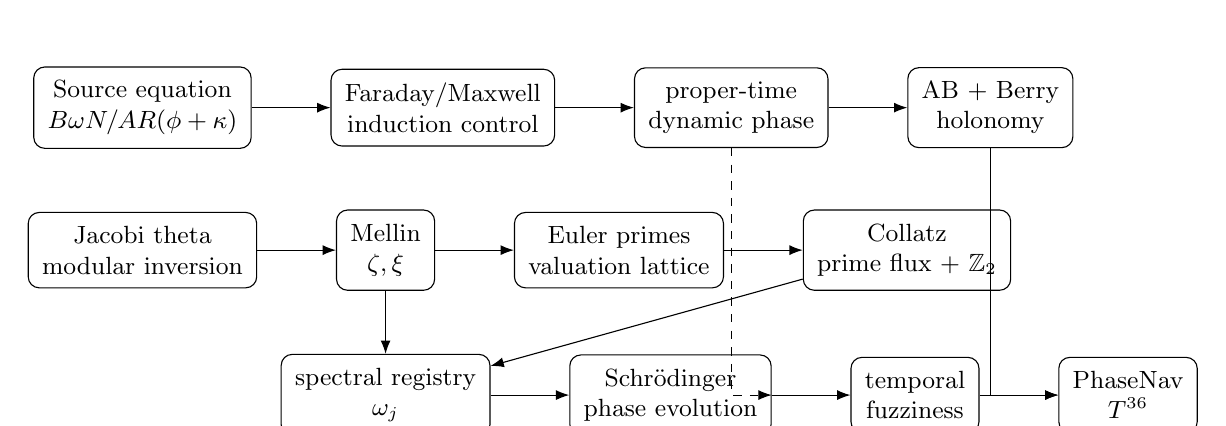
\begin{tikzpicture}[node distance=8mm and 10mm,>=Latex,every node/.style={draw,rounded corners,align=center,font=\small,inner sep=5pt}]
\node (src) {Source equation\\\(B\omega N/AR\)(\(\phi+\kappa\))};
\node[right=of src] (em) {Faraday/Maxwell\\induction control};
\node[right=of em] (proper) {proper-time\\dynamic phase};
\node[right=of proper] (hol) {AB + Berry\\holonomy};
\node[below=of src] (theta) {Jacobi theta\\modular inversion};
\node[right=of theta] (zeta) {Mellin\\\(\zeta,\xi\)};
\node[right=of zeta] (prime) {Euler primes\\valuation lattice};
\node[right=of prime] (collatz) {Collatz\\prime flux + \(\mathbb Z_2\)};
\node[below=of zeta] (spec) {spectral registry\\\(\omega_j\)};
\node[right=of spec] (sch) {Schrödinger\\phase evolution};
\node[right=of sch] (fuzz) {temporal\\fuzziness};
\node[right=of fuzz] (t36) {PhaseNav\\\(T^{36}\)};
\draw[->] (src)--(em); \draw[->] (em)--(proper); \draw[->] (proper)--(hol);
\draw[->] (theta)--(zeta); \draw[->] (zeta)--(prime); \draw[->] (prime)--(collatz);
\draw[->] (zeta)--(spec); \draw[->] (collatz)--(spec); \draw[->] (spec)--(sch); \draw[->] (sch)--(fuzz); \draw[->] (fuzz)--(t36);
\draw[->] (hol) |- (t36);
\draw[->,dashed] (proper) |- (sch);
\end{tikzpicture}
\end{center}

The solid arrows denote defined or standard structural maps. Dashed arrows denote a parameter-binding interface that is permitted only when units and physical semantics are declared. No arrow in this diagram is a proof that the domains are physically identical.

\subsection{Three merge points}

The first merge point is \emph{phase}: electromagnetic potentials, dynamic phase, Berry phase, Mellin characters, and Collatz parity holonomy can all be represented as phases, but they retain distinct provenance.

The second merge point is \emph{holonomy}: closed transport can produce a non-trivial group element even when the local endpoint coordinate returns to its start.

The third merge point is \(\Tthirtysix\): PhaseNav can host multiple phase channels in one explicit torus state while preserving exact arithmetic/provenance outside the float-angle realisation.

\section{Physical phase branch: induction, proper time, Unruh, Aharonov--Bohm, Berry, Euler}

\subsection{Faraday and Maxwell as the classical control layer}

For a coil with \(N\) turns and magnetic flux \(\Phi_B\), Faraday's law gives
\begin{equation}
\boxed{\mathcal E=-N\frac{d\Phi_B}{dt}.}
\end{equation}
For the idealised rotating-flux control
\begin{equation}
\Phi_B(t)=BA\cos(\omega t+\phi),
\end{equation}
one obtains
\begin{equation}
\boxed{\mathcal E(t)=NAB\omega\sin(\omega t+\phi).}
\label{eq:faraday-rot}
\end{equation}
Status: \status{STANDARD\_EXACT} under the stated idealisation. Equation~\eqref{eq:faraday-rot} explains why a product containing \(B\omega N\) is natural in a rotating magnetic generator. It does \emph{not} make the source equation~\eqref{eq:source-zpe} identical to Faraday's law: Faraday contains a flux geometry and a derivative-generated trigonometric factor.

Maxwell's field-energy density supplies the ordinary electromagnetic baseline,
\begin{equation}
 u_{\rm EM}=\frac{\epsilon_0}{2}|\mathbf E|^2+\frac{1}{2\mu_0}|\mathbf B|^2.
\end{equation}
Any generator experiment must first close mechanical input, electromagnetic storage, ohmic loss, eddy currents, magnetic hysteresis, switching losses, and measured output before assigning a residual to a new channel.

\subsection{Quantum zero-point scale}

For a quantum harmonic oscillator,
\begin{equation}
E_n=\hbar\omega\left(n+\frac12\right),
\qquad
\boxed{E_0=\frac12\hbar\omega}.
\end{equation}
Status: \status{STANDARD\_EXACT}. This establishes a vacuum-ground-state energy scale in the oscillator model. It does not establish an extractable net-energy source. In this monograph, ``ZPE'' is therefore retained as source genealogy and as a research target, not as a closed energy-balance result.

\subsection{Dynamic phase and proper time}

For a local energy eigencomponent transported along proper time \(\tau\),
\begin{equation}
\boxed{d\varphi_{\rm dyn}=-\frac{E_{\rm loc}}{\hbar}\,d\tau.}
\label{eq:dynphase}
\end{equation}
For a worldline,
\begin{equation}
 d\tau=\frac1c\sqrt{-g_{\mu\nu}dx^\mu dx^\nu}
\end{equation}
for the mostly-plus convention. In a static metric one may write \(d\tau=N_g\,dt\), where \(N_g\) is the gravitational lapse for the chosen observer. The corresponding stationary redshift relation is conventionally represented as
\begin{equation}
 E_{\rm loc}=\frac{E_\infty}{N_g}.
\end{equation}
The invariant phase accounting prevents a redshift relation from becoming an energy-extraction rule by algebra alone.

PNCS v0.27 already contains a separate computational \emph{phase proper time}. Its current contract explicitly states that laboratory time is not modified. The present monograph preserves that boundary.

\subsection{Acceleration and the Unruh scale}

Uniform proper acceleration \(a\) defines the Unruh temperature
\begin{equation}
\boxed{T_U=\frac{\hbar a}{2\pi c k_B}},
\qquad
k_BT_U=\frac{\hbar a}{2\pi c}.
\end{equation}
Status: \status{STANDARD\_EXACT} in quantum field theory for the idealised uniformly accelerated detector setting \cite{Unruh1976}. The associated angular-frequency scale is
\begin{equation}
\omega_U=\frac{k_BT_U}{\hbar}=\frac{a}{2\pi c}.
\end{equation}
This provides a precise acceleration--frequency bridge. It is not a free-energy mechanism; the accelerated detector problem includes the work/interaction required to maintain acceleration.

\subsection{Aharonov--Bohm phase}

For a charged particle, the electromagnetic contribution to phase can be written, in a standard non-covariant split,
\begin{equation}
\boxed{
\Delta\varphi_{\rm AB}
=\frac{q}{\hbar}
\left(
\int \mathbf A\cdot d\mathbf l
-\int V\,dt
\right).
}
\end{equation}
For a closed magnetic Aharonov--Bohm loop,
\begin{equation}
\Delta\varphi_{\rm AB}=\frac{q}{\hbar}\oint\mathbf A\cdot d\mathbf l
=\frac{q\Phi_B}{\hbar}.
\end{equation}
The physical point is that a measurable interference phase can depend on gauge-potential holonomy even when the particle paths lie in a region of vanishing local magnetic field \cite{AharonovBohm1959}.

\subsection{Berry phase and geometric holonomy}

For a non-degenerate instantaneous eigenstate \(|n(\lambda)\rangle\), define the Berry connection
\begin{equation}
\mathcal A_a(\lambda)=i\langle n(\lambda)|\partial_{\lambda^a}n(\lambda)\rangle.
\end{equation}
For an adiabatically closed parameter loop \(C\),
\begin{equation}
\boxed{\gamma_B[C]=\oint_C\mathcal A_a\,d\lambda^a.}
\end{equation}
Its curvature is
\begin{equation}
\mathcal F=d\mathcal A,
\end{equation}
and, when the gauge patch permits,
\begin{equation}
\gamma_B=\int_\Sigma\mathcal F.
\end{equation}
Status: \status{STANDARD\_EXACT} for the usual adiabatic construction \cite{Berry1984}.

\subsection{Combined phase connection}

A convenient bookkeeping one-form is
\begin{equation}
\boxed{
\Gamma
= -\frac{E_{\rm loc}}{\hbar}d\tau
+\frac{q}{\hbar}A_\mu dx^\mu
+\mathcal A_a d\lambda^a,
}
\label{eq:combined-connection}
\end{equation}
with signs dependent on the electromagnetic four-potential convention. The corresponding holonomy is
\begin{equation}
\boxed{U[C]=\exp\left(i\oint_C\Gamma\right)}
\end{equation}
for an Abelian single-component case; non-Abelian transport requires path ordering.

\INTERP
Equation~\eqref{eq:combined-connection} motivates a PhaseNav principle: a state may carry physically or mathematically relevant information in the transport history, not only in a local endpoint coordinate. The interpretation is \emph{not} that gravitational, electromagnetic, Berry, and arithmetic connections are the same physical field. They are distinct connections that can share a transport/holonomy representation.

\subsection{Euler closure and the \((1,-1)\) sign pair}

Euler's identity gives
\begin{equation}
\boxed{e^{i\pi}=-1},\qquad e^{i2\pi}=+1.
\end{equation}
A loop with total phase \(\pi\pmod{2\pi}\) therefore returns the scalar holonomy \(-1\), while a double traversal gives \(+1\). Berry's original analysis includes sign reversal around certain degeneracies and relates geometric phase to familiar spinor sign behaviour \cite{Berry1984}.

\INTERP
The project uses the pair \((+1,-1)\) as a minimal two-valued holonomy representation. Whenever an arithmetic construction below exhibits one-loop \(-1\) and two-loop \(+1\), that is a representation-theoretic analogy to double-cover closure, not evidence that the arithmetic degree of freedom is physical spin.

\section{Theta--zeta branch: modular inversion, Mellin scale, completion, and primes}

\subsection{Jacobi theta modular inversion}

Define
\begin{equation}
\vartheta(t)=\sum_{n\in\mathbb Z}e^{-\pi n^2t},\qquad t>0.
\end{equation}
The modular inversion is
\begin{equation}
\boxed{\vartheta(t)=t^{-1/2}\vartheta(1/t).}
\label{eq:theta-modular}
\end{equation}
Status: \status{STANDARD\_EXACT} \cite{DLMFTheta}. Introduce \(u=\log t\). Then multiplicative inversion becomes additive reflection \(u\mapsto-u\). A symmetrised profile can therefore be chosen even in log-scale.

\subsection{Mellin transform to zeta}

A standard theta Mellin relation yields the gamma--zeta factor; one convenient normalisation is
\begin{equation}
\boxed{
\int_0^\infty[\vartheta(t)-1]t^{s/2-1}\,dt
=2\pi^{-s/2}\Gamma(s/2)\zeta(s),
\qquad \RePart(s)>1.
}
\label{eq:theta-mellin}
\end{equation}
Equivalent theta-function Mellin formulae are tabulated by DLMF \cite{DLMFThetaMellin}.

For \(t=e^u\), Mellin kernels take the form
\begin{equation}
 t^{-s}=e^{-su}=e^{-\sigma u}e^{-i\tau u},
\qquad s=\sigma+i\tau.
\end{equation}
Thus the imaginary part of \(s\) is a Fourier-like phase frequency conjugate to logarithmic scale.

\subsection{Completed zeta and the half-axis}

Define
\begin{equation}
\xi(s)=\frac12s(s-1)\pi^{-s/2}\Gamma(s/2)\zeta(s).
\end{equation}
Then
\begin{equation}
\boxed{\xi(s)=\xi(1-s).}
\label{eq:xi-reflection}
\end{equation}
Status: \status{STANDARD\_EXACT} \cite{DLMFZetaReflection}. Because \(\xi(\bar s)=\overline{\xi(s)}\), the anti-linear involution
\begin{equation}
J(s)=1-\bar s
\end{equation}
has fixed set
\begin{equation}
\boxed{J(s)=s\iff \RePart(s)=\frac12.}
\end{equation}
This fixed-set statement does not prove that all non-trivial zeros lie on that set.

\subsection{Euler product and the prime alphabet}

For \(\RePart(s)>1\),
\begin{equation}
\boxed{\zeta(s)=\prod_{p\in\mathbb P}(1-p^{-s})^{-1}.}
\label{eq:euler-product}
\end{equation}
Status: \status{STANDARD\_EXACT} \cite{DLMFZetaEuler}. Every positive integer has a unique prime-valuation vector
\begin{equation}
\mathbf v(n)=\{v_p(n)\}_{p\in\mathbb P},
\qquad
n=\prod_p p^{v_p(n)},
\end{equation}
and therefore
\begin{equation}
\boxed{\log n=\sum_p v_p(n)\log p.}
\label{eq:prime-log}
\end{equation}
Only finitely many terms are non-zero for any fixed integer.

This identifies a common multiplicative coordinate system. Zeta packages independent prime powers through the Euler product in its convergence half-plane; Collatz, developed in the next branch, generates a deterministic trajectory through the same integer valuation lattice.

\subsection{Critical-line prime characters}

For a single prime and \(s=\tfrac12+i\tau\),
\begin{equation}
\boxed{p^{-s}=p^{-1/2}e^{-i\tau\log p}.}
\label{eq:prime-critical-character}
\end{equation}
Thus a finite prime character has amplitude \(p^{-1/2}\) and phase \(-\tau\log p\). This identity is valid for an individual finite factor for any complex \(s\).

\begin{claim}{Convergence boundary -- \status{MANDATORY}.}
Equation~\eqref{eq:euler-product} is a directly convergent infinite product only for \(\RePart(s)>1\). The project must not numerically multiply an unregularised infinite Euler product on \(\RePart(s)=1/2\) and call the result \(\zeta(s)\). Critical-line work must use the analytically continued \(\zeta/\xi\) or explicitly finite, receipt-bound prime-mode truncations.
\end{claim}

\INTERP
The prime representation supplies the missing multiplicative ``alphabet'' between zeta and Collatz. It closes a representation bridge: both systems can be expressed using \(\log p\) and \(v_p\). It does not yet close a spectral identity between the Riemann operator sought by Hilbert--P\'olya-type programmes and a Collatz transfer/Koopman operator.

\section{Collatz prime-flow branch: exact cocycle, prime flux, and holonomy}

\subsection{Shortcut Collatz map}

Define
\begin{equation}
C(n)=
\begin{cases}
n/2,&n\equiv0\pmod2,\\[2mm]
(3n+1)/2,&n\equiv1\pmod2,
\end{cases}
\qquad n\in\mathbb N_{>0}.
\end{equation}
For a valid step \(n_k\to n_{k+1}=C(n_k)\), define
\begin{equation}
r_k=\frac{n_{k+1}}{n_k},
\qquad
b_k=n_k\bmod2\in\{0,1\}.
\end{equation}
The implementation stores \(r_k\) first as an exact reduced rational.

\subsection{The \(\mathbb Z_2\) branch representation}

The non-trivial one-dimensional unitary representation of \(\mathbb Z_2\) is
\begin{equation}
\boxed{\rho(b)=(-1)^b=e^{i\pi b}.}
\end{equation}
Define the Mellin-sign step cocycle
\begin{equation}
\boxed{w_s(n_k)=r_k^{-s}(-1)^{b_k}.}
\label{eq:step-cocycle}
\end{equation}
For \(s=\sigma+i\tau\),
\begin{equation}
|w_s|=r_k^{-\sigma},
\qquad
\arg w_s=-\tau\log r_k+\pi b_k\pmod{2\pi}.
\end{equation}
Status: \status{PROJECT\_EXACT} after definition.

\subsection{Orbit factorisation theorem}

Let
\begin{equation}
\mathcal O_m=(n_0,n_1,\ldots,n_m),
\qquad n_{k+1}=C(n_k),
\end{equation}
and
\begin{equation}
W_s(\mathcal O_m)=\prod_{k=0}^{m-1}w_s(n_k),
\qquad
N_{\rm odd}=\sum_{k=0}^{m-1}b_k.
\end{equation}
Then
\begin{equation}
\boxed{
W_s(\mathcal O_m)
=
\left(\frac{n_m}{n_0}\right)^{-s}
(-1)^{N_{\rm odd}}.
}
\label{eq:orbit-factor}
\end{equation}
Status: \status{PROJECT\_EXACT}. The proof is the telescoping product
\begin{equation}
\prod_{k<m}\frac{n_{k+1}}{n_k}=\frac{n_m}{n_0}
\end{equation}
combined with multiplication of the parity signs.

\subsection{Complementary defect and the half-axis}

Set
\begin{equation}
L=\log\frac{n_m}{n_0}.
\end{equation}
From \eqref{eq:orbit-factor},
\begin{equation}
\log|W_s|=-\sigma L,
\qquad
\log|W_{1-s}|=-(1-\sigma)L.
\end{equation}
Define
\begin{equation}
\boxed{
D_C(s;\mathcal O_m)
=
\big(\log|W_s|-\log|W_{1-s}|\big)^2
=(2\sigma-1)^2L^2.
}
\label{eq:collatz-defect}
\end{equation}
For a non-closed path \(L\neq0\),
\begin{equation}
\boxed{D_C=0\iff \RePart(s)=\frac12.}
\end{equation}
For a closed path \(L=0\), \(D_C=0\) for every \(s\). Closed paths are therefore degenerate controls and cannot serve as evidence that the half-axis is uniquely selected.

\subsection{Critical-line conjugate pair}

For \(s=\tfrac12+i\tau\),
\begin{equation}
\boxed{W_{1-s}=\overline{W_s}.}
\end{equation}
This is the exact origin of an 18-pair \(\Tthirtysix\) construction used below.

\subsection{Prime-valuation flux}

Define the stepwise prime flux
\begin{equation}
\boxed{\Delta v_{p,k}=v_p(n_{k+1})-v_p(n_k).}
\label{eq:prime-flux}
\end{equation}
By unique factorisation,
\begin{equation}
\boxed{r_k=\prod_p p^{\Delta v_{p,k}},}
\qquad
\log r_k=\sum_p\Delta v_{p,k}\log p.
\end{equation}
Hence the exact step cocycle factorises prime by prime:
\begin{equation}
\boxed{
w_s(n_k)
=(-1)^{b_k}\prod_p p^{-s\Delta v_{p,k}}.
}
\label{eq:prime-cocycle}
\end{equation}
For the full orbit define
\begin{equation}
\Delta V_p=\sum_{k<m}\Delta v_{p,k}=v_p(n_m)-v_p(n_0).
\end{equation}
Then
\begin{equation}
\boxed{
W_s(\mathcal O_m)=(-1)^{N_{\rm odd}}\prod_p p^{-s\Delta V_p}.
}
\label{eq:prime-orbit}
\end{equation}
Only finitely many \(\Delta V_p\) are non-zero for a finite endpoint pair.

On the critical line, the orbit phase becomes
\begin{equation}
\boxed{
\Theta_{\mathcal O}(\tau)
=
\pi N_{\rm odd}
-	au\sum_p\Delta V_p\log p
\pmod{2\pi}.
}
\label{eq:prime-phase}
\end{equation}
Thus
\begin{equation}
\Theta_{\mathcal O}=\Theta_{\mathbb Z_2}+\Theta_{\rm prime}.
\end{equation}

\subsection{Closed-cycle cancellation of prime flux}

If \(n_m=n_0\), then \(\Delta V_p=0\) for every prime, so
\begin{equation}
\Theta_{\rm prime}=0,
\qquad
\boxed{W_s=(-1)^{N_{\rm odd}}.}
\end{equation}
For the control cycle
\begin{equation}
1\to2\to1,
\end{equation}
there is one odd source state, so
\begin{equation}
\boxed{W_s=-1=e^{i\pi}.}
\end{equation}
Two traversals give \(+1\). The one-loop/double-loop closure is therefore exact for the defined sign cocycle.

\subsection{Where the non-trivial prime interaction resides}

The even branch \(n\mapsto n/2\) is multiplicative and transparent in valuation coordinates. The odd branch contains
\begin{equation}
3n+1,
\end{equation}
and addition prevents factorwise separation:
\begin{equation}
v_p(3n+1)\neq v_p(3)+v_p(n)
\end{equation}
in general. Thus the map
\begin{equation}
\mathbf v(n)\mapsto\mathbf v(3n+1)-\mathbf e_2
\end{equation}
is an arithmetic coupling of prime channels.

\INTERP
Zeta's Euler product represents free multiplicative composition of prime powers in its convergence region, whereas the Collatz odd branch deterministically re-couples prime valuations through the additive operation \(3n+1\). This is a useful physical-style analogy (``free modes'' versus ``interaction vertex''), not a theorem identifying a quantum field theory with Collatz arithmetic.

\subsection{Weighted Koopman operator}

Define, on a declared function space of observables,
\begin{equation}
\boxed{(U_s f)(n)=w_s(n)f(C(n)).}
\end{equation}
Then
\begin{equation}
U_s^m f(n_0)=W_s(\mathcal O_m)f(n_m).
\end{equation}
Operator approaches to the \(3x+1\) system, including Koopman methods and Fourier analysis of sign sequences, exist independently in the literature \cite{LeventidesPoulios2020}. The specific Mellin-sign cocycle and prime-flux PhaseNav embedding in this monograph are project constructions.

\section{Zeta--Schrödinger temporal branch: spectral synthesis, phase dispersion, and fuzziness}

\subsection{Why the transform must be specified}

A discrete Fourier transform/FFT assumes samples on a uniform frequency or time grid according to the chosen convention. Prime logarithms \(\log p\) and non-trivial zeta-zero ordinates are not uniformly spaced. Therefore the canonical project language is:
\begin{itemize}[leftmargin=2em]
\item uniform registry \(\Rightarrow\) DFT/FFT may be used;
\item non-uniform registry \(\Rightarrow\) direct Fourier synthesis or a declared NUFFT implementation;
\item gridding/interpolation \(\Rightarrow\) a separate approximation receipt is mandatory.
\end{itemize}
The phrase ``temporal FFT'' is therefore an implementation shortcut, not a mathematical identity between zeta and time.

\subsection{Spectral registries}

A temporal synthesis experiment begins with a content-addressed registry
\begin{equation}
\Omega=\{(\omega_j,c_j,\mathsf{source}_j)\}_{j=1}^{M}.
\end{equation}
Allowed source classes include:
\begin{enumerate}[leftmargin=2em]
\item \status{UNIFORM\_CONTROL}: a preregistered uniform frequency grid;
\item \status{PRIME\_LOG}: \(\omega_j=\Omega_0\log p_j\) for a finite prime set;
\item \status{ZETA\_ZERO\_ORDINATE}: \(\omega_j=\Omega_0\gamma_j\) for declared non-trivial zero ordinates \(\gamma_j\), used only as a diagnostic registry;
\item \status{COLLATZ\_OPERATOR\_SPECTRUM}: eigenfrequencies of a fully specified finite or mathematically controlled operator;
\item \status{EXTERNAL\_MEASUREMENT}: an experimental spectrum with provenance.
\end{enumerate}
No registry is canonical merely because it produces an attractive waveform.

\subsection{Schrödinger phase evolution}

Define a diagonal project Hamiltonian on the declared modes,
\begin{equation}
\boxed{\hat H_{ZC}|j\rangle=E_j|j\rangle,
\qquad E_j=\hbar\omega_j.}
\end{equation}
For
\begin{equation}
|\Psi(0)\rangle=\sum_j c_j|j\rangle,
\qquad\sum_j|c_j|^2=1,
\end{equation}
unitary evolution is
\begin{equation}
\boxed{
|\Psi(\tau)\rangle
=\sum_j c_j e^{-i\omega_j\tau}|j\rangle.
}
\label{eq:sch-evolution}
\end{equation}
The parameter is written \(\tau\) deliberately. It may be ordinary laboratory time in a standard Hamiltonian simulation, proper time for a physical local clock, or PNCS phase proper time in the computational substrate. Those meanings must never be silently exchanged.

A single eigenmode acquires only a global phase and has no internal relative-phase clock. At least two distinct \(\omega_j\) are required for non-trivial internal phase relations.

\subsection{Temporal synthesis}

Define the coherent temporal amplitude
\begin{equation}
\boxed{x(\tau)=\sum_{j=1}^{M}c_j e^{-i\omega_j\tau}.}
\label{eq:temporal-synthesis}
\end{equation}
For uniformly spaced frequencies this can be sampled efficiently by inverse FFT under a declared convention. For non-uniform \(\omega_j\), equation~\eqref{eq:temporal-synthesis} itself is the authority and may be evaluated directly or via NUFFT.

For finite prime-log modes,
\begin{equation}
\omega_p=\Omega_0\log p
\end{equation}
gives
\begin{equation}
\boxed{x(\tau)=\sum_{p\in P}c_p\,p^{-i\Omega_0\tau}.}
\label{eq:prime-time}
\end{equation}
Combining this with a critical-line finite prime character gives
\begin{equation}
p^{-1/2-i\Omega_0\tau}=p^{-1/2}e^{-i\Omega_0\tau\log p}.
\end{equation}
This is a finite-mode amplitude/phase identity, not use of the divergent critical-line Euler product.

\subsection{Definition of Zeta--Schrödinger fuzziness}

Let
\begin{equation}
p_j=|c_j|^2,
\qquad \sum_jp_j=1.
\end{equation}
Define the survival/coherence amplitude
\begin{equation}
\boxed{
A_Z(\tau)
=\langle\Psi(0)|\Psi(\tau)\rangle
=\sum_jp_j e^{-i\omega_j\tau}.
}
\label{eq:az}
\end{equation}
The project-defined \emph{Zeta--Schrödinger temporal fuzziness} is
\begin{equation}
\boxed{
\mathcal F_Z(\tau)=1-|A_Z(\tau)|^2.
}
\label{eq:fuzziness}
\end{equation}
Status: \status{PROJECT\_EXACT} as a definition. It satisfies
\begin{equation}
0\le \mathcal F_Z\le1,
\qquad
\mathcal F_Z(0)=0.
\end{equation}
For a one-mode state, \(\mathcal F_Z(\tau)=0\) for all \(\tau\).

\subsection{Small-time expansion}

Let
\begin{equation}
\bar\omega=\sum_jp_j\omega_j,
\qquad
(\Delta\omega)^2=\sum_jp_j(\omega_j-\bar\omega)^2.
\end{equation}
Expanding equation~\eqref{eq:az} gives
\begin{equation}
\boxed{
|A_Z(\tau)|^2
=1-(\Delta\omega)^2\tau^2+O(\tau^4),
}
\end{equation}
and hence
\begin{equation}
\boxed{
\mathcal F_Z(\tau)
=(\Delta\omega)^2\tau^2+O(\tau^4).
}
\label{eq:fuzz-small}
\end{equation}
Equivalently \(\Delta E=\hbar\Delta\omega\) controls the initial rate at which the state becomes distinguishable from its initial ray.

\subsection{Relative phase as an operational clock}

For two modes,
\begin{equation}
\Delta\varphi_{12}(\tau)
=(\omega_2-\omega_1)\tau.
\end{equation}
The measurable internal change is relative phase, not the common global phase. A project clock observable may therefore be built from a vector of pairwise phase differences or from \(\mathcal F_Z\), with revivals explicitly allowed.

\INTERP
The phrase ``fuzziness makes time flow'' is sharpened here to the following candidate statement: \emph{operational temporal change is available when a spectral superposition develops non-trivial relative phases, and \(\mathcal F_Z\) measures loss of initial phase coherence}. This is compatible with standard unitary quantum dynamics. The stronger ontological claim that physical time itself is generated by zeta/Collatz spectral fuzziness remains \status{OPEN}.

\subsection{Local proper-time binding}

A physically local form replaces the evolution parameter by proper time,
\begin{equation}
|\Psi(\tau_{\rm phys})\rangle
=\sum_jc_j e^{-i\omega_j\tau_{\rm phys}}|j\rangle.
\end{equation}
A PNCS runtime form may instead use the v0.27 content-addressed phase proper time,
\begin{equation}
|\Psi(\tau_{\rm PNCS})\rangle
=\sum_jc_j e^{-i\omega_j\tau_{\rm PNCS}}|j\rangle,
\end{equation}
with the mandatory receipt field
\begin{center}
\texttt{laboratory\_time\_modified = false}.
\end{center}
The two equations have the same numerical form but different semantics and provenance.

\subsection{Revivals are features, not failures}

Because equation~\eqref{eq:fuzziness} is generated by coherent phases, \(\mathcal F_Z\) need not increase monotonically. Finite commensurate spectra can exhibit exact revivals; generic incommensurate finite spectra can exhibit approximate recurrences. Therefore the project must not equate ``time arrow'' with monotonic fuzziness without an additional open-system/decoherence model.

\section{PhaseNav \(T^{36}\) implementation architecture and validation gates}

\subsection{Two distinct 36D embeddings}

The project must distinguish two useful embeddings.

\paragraph{PAIR18 embedding.}
For a finite Collatz path with
\begin{equation}
L=\log(n_m/n_0),
\end{equation}
and an explicit registry \(\boldsymbol\tau=(\tau_1,\ldots,\tau_{18})\), define
\begin{align}
\theta_{2j-1}&=\pi N_{\rm odd}-\tau_jL\pmod{2\pi},\\
\theta_{2j}&=\pi N_{\rm odd}+\tau_jL\pmod{2\pi},
\qquad j=1,\ldots,18.
\end{align}
Then
\begin{equation}
\boxed{\boldsymbol\theta_{\rm pair}\in T^{36}.}
\end{equation}
This is the exact critical-line complementary-pair embedding inherited from v0.1.

For a closed odd-parity cycle \(L=0\),
\begin{equation}
\boldsymbol\theta_{\rm pair}=(\pi,\ldots,\pi),
\end{equation}
and after double traversal,
\begin{equation}
\boldsymbol\theta_{\rm pair}=(0,\ldots,0)\pmod{2\pi}.
\end{equation}

\paragraph{MODE36 embedding.}
For a direct temporal registry of 36 modes,
\begin{equation}
\theta_j(\tau)=\theta_j(0)-\omega_j\tau\pmod{2\pi},
\qquad j=1,\ldots,36.
\end{equation}
This embedding is appropriate for temporal synthesis and fuzziness. It is not automatically equivalent to PAIR18. A bridge between them requires an explicit registry map.

\subsection{State separation}

The runtime must keep at least three layers separate:
\begin{enumerate}[leftmargin=2em]
\item \textbf{exact arithmetic state}: integers, rationals, branch word, prime valuations, endpoint ratio;
\item \textbf{spectral state}: source-labelled \(\omega_j\), amplitudes/weights, precision and transform policy;
\item \textbf{phase realisation}: float or high-precision angles on \(T^{36}\), phase proper time, and numerical backend.
\end{enumerate}
A float-angle hash may not replace exact arithmetic identity.

\subsection{Proposed experimental native paths}

The monograph recommends the following non-promoting native families:
\begin{lstlisting}[basicstyle=\ttfamily\small,frame=single,breaklines=true]
TZC.THETA_MODULAR_INVERSION
TZC.THETA_MELLIN
TZC.XI_REFLECTION
TZC.PRIME_VALUATION
TZC.COLLATZ_SHORTCUT
TZC.PRIME_FLUX
TZC.Z2_SIGN
TZC.MELLIN_CHARACTER
TZC.STEP_WEIGHT
TZC.ORBIT_FACTORIZATION
TZC.SELF_DUAL_DEFECT
TZC.CRITICAL_PAIR
TZC.T36_PAIR_PROJECTION

ZST.SPECTRAL_REGISTRY
ZST.TEMPORAL_SYNTHESIS
ZST.SCHRODINGER_PHASE
ZST.COHERENCE_AMPLITUDE
ZST.TEMPORAL_FUZZINESS
ZST.T36_MODE_PROJECTION
ZST.PHASE_PROPER_TIME_BIND
\end{lstlisting}
All remain \texttt{EPISTEMIC CHYBA / MODE READ\_ONLY} until separately admitted.

\subsection{Reference module decomposition}

A future implementation should be split rather than placed in one file:
\begin{lstlisting}[basicstyle=\ttfamily\small,frame=single,breaklines=true]
src/phasenav_natural_code/
  theta_zeta_core.py
  collatz_prime_flux.py
  zeta_schrodinger_time.py
  holonomy_t36.py
\end{lstlisting}
The standard theta/zeta numerical functions must not contain Collatz semantics. Exact Collatz arithmetic must not depend on numerical zeta-zero tables. Temporal synthesis must receive its spectral registry as explicit input.

\subsection{Fail-closed input contract}

Reject or quarantine:
\begin{itemize}[leftmargin=2em]
\item non-positive Collatz integers;
\item booleans supplied as integers;
\item unbounded iteration;
\item excessive integer bit-length beyond declared bounds;
\item non-finite complex parameters or frequencies;
\item implicit zeta-zero downloads;
\item a prime-log critical-line calculation that silently evaluates the divergent Euler product;
\item a 36D build with the wrong number of coordinates;
\item transform results whose grid/interpolation provenance is missing;
\item any request for external effects from the pure mathematical core.
\end{itemize}

\subsection{Validation gates}

\begin{longtable}{p{0.13\linewidth}p{0.78\linewidth}}
\toprule
Gate & Required evidence\\
\midrule
A & Jacobi theta modular inversion and theta--Mellin--zeta controls at declared precision.\\
B & Exact shortcut Collatz step and rational-ratio controls.\\
C & Direct vs endpoint-factorised Mellin-sign orbit weights across frozen seeds/probes.\\
D & Prime-valuation reconstruction: \(n=\prod p^{v_p(n)}\), step ratio from \(\Delta v_p\), and orbit endpoint flux.\\
E & Self-dual defect equals \((2\sigma-1)^2L^2\); non-closed half-axis control and closed-path degeneracy control.\\
F & Critical-line conjugate pair relation and 18-pair \(T^{36}\) geometry.\\
G & One-loop \(-1\), double-loop \(+1\) control cycle.\\
H & Temporal synthesis: direct DFT agrees with FFT on uniform grids; non-uniform registry remains on direct/NUFFT path.\\
I & Fuzziness invariants: \(\mathcal F_Z(0)=0\), \(0\le\mathcal F_Z\le1\), single-mode zero, two/multi-mode analytic controls, small-time variance law.\\
J & Exact arithmetic identities remain unchanged when numerical precision/backend changes; only realisation receipts may differ.\\
K & If bound to PNCS v0.27, semantic projection remains unchanged and \texttt{laboratory\_time\_modified=false}.\\
\bottomrule
\end{longtable}

\subsection{Fresh v0.2 reference validation}

A standalone reference suite accompanies the local build of this monograph. It tests the exact v0.1 identities plus the new prime-flux and temporal-fuzziness layer. Fresh result: \textbf{33/33 checks PASS}. The direct-versus-factorised Collatz weight sweep covered seeds 1--400 with four complex probes; the maximum complex-weight disagreement was approximately \(4.79\times10^{-12}\), consistent with the declared floating realisation. Prime-flux reconstruction was checked exactly with rational arithmetic over 7,500 Collatz steps. The suite also verified uniform FFT/direct-DFT equivalence, fuzziness bounds, the one-mode zero-fuzziness control, a two-mode analytic identity, and the small-time variance law.\par
\medskip
Validation report SHA-256: \texttt{79d3aeeeb639fec2de207c769e19fb4a23dcc81613f531919f5de2ae257a4a52}. This report is a \status{NUMERICAL\_CONTROL}, not promotion of the open bridges.

\subsection{Scientific falsification criteria}

The module must retain negative results. A candidate bridge is rejected or downgraded if:
\begin{enumerate}[leftmargin=2em]
\item it requires fitting a parameter after inspecting known zeta zeros;
\item a proposed ``Collatz zeta'' depends materially on an arbitrary truncation boundary with no controlled limit;
\item the prime-valuation representation fails to reproduce the exact endpoint ratio;
\item off-axis zeros of the finite-path defect occur for non-closed paths;
\item a temporal result depends on confusing a non-uniform spectrum with a standard FFT;
\item fuzziness is reported as monotonic when revivals are present;
\item a phase-proper-time simulation is promoted to laboratory-time modification;
\item an energy residual is reported before the conventional electromagnetic/mechanical balance is closed.
\end{enumerate}

\section{Open bridges, branch-specific research programme, and promotion criteria}

\subsection{What is now closed at the representation level}

The following chain is mathematically controlled:
\begin{equation}
\boxed{
\vartheta
\xrightarrow{\rm Mellin}
\zeta/\xi
\xrightarrow{\rm Euler\;coordinates}
\{v_p,\log p\}
\xleftarrow{\rm exact\;factorisation}
\text{Collatz prime flow}.
}
\end{equation}
The right-hand arrow is a common-coordinate bridge, not an equality of operators. The exact Collatz branch further provides
\begin{equation}
\boxed{
\mathcal O_m
\longrightarrow
W_s
\longrightarrow
D_C
\longrightarrow
\text{critical conjugate pairs}
\longrightarrow
T^{36}.
}
\end{equation}
The temporal branch provides
\begin{equation}
\boxed{
\Omega
\longrightarrow
\hat H_{ZC}
\longrightarrow
|\Psi(\tau)\rangle
\longrightarrow
A_Z(\tau)
\longrightarrow
\mathcal F_Z(\tau).
}
\end{equation}

\subsection{The remaining hard zeta--Collatz bridge}

The principal mathematical question is now sharply stated:
\begin{quote}
Does a non-arbitrary infinite-dimensional Collatz operator, defined on a mathematically natural function space and using the exact prime/Mellin cocycle or a derived intrinsic weighting, possess a spectral invariant whose analytic continuation and reflection structure are provably related to \(\xi(s)\)?
\end{quote}
A suggestive target has the schematic form
\begin{equation}
\det_{\rm reg}(I-\mathcal L_C(s))
\stackrel{?}{\longleftrightarrow}
\xi(s),
\end{equation}
but the determinant class, function space, regularisation, and weighting must be derived rather than chosen to fit the answer. Until those are fixed, this equation is \status{OPEN}.

\subsection{The remaining time bridge}

The operational phase-dispersion model is closed by definition and standard unitary evolution. The ontological statement
\begin{equation}
\text{``physical time flows because zeta--Schrödinger fuzziness is non-zero''}
\end{equation}
is \status{OPEN}. To promote it beyond interpretation requires a physical model in which:
\begin{enumerate}[leftmargin=2em]
\item the spectral registry is generated by measured or derived physical degrees of freedom rather than selected numerically;
\item the same \(\mathcal F_Z\) predicts independent clock/interference observables;
\item competing standard models are quantitatively compared;
\item the model survives blinded prospective tests.
\end{enumerate}

\subsection{The remaining gravity/Unruh bridge}

The standard relations
\begin{equation}
d\varphi=-E\,d\tau/\hbar,
\qquad
T_U=\hbar a/(2\pi c k_B)
\end{equation}
provide legitimate phase/proper-time and acceleration/frequency structures. A PhaseNav claim that the arithmetic spectrum controls a physical Unruh detector response requires a concrete coupling Hamiltonian and predicted detector transition rate. It is currently \status{OPEN}.

\subsection{The remaining electromagnetic/ZPE bridge}

The classical generator baseline is governed by Maxwell--Faraday dynamics and measured power accounting. The quantum oscillator provides a zero-point scale. The project source equation preserves an intended phase/information modulation. A physical ZPE extraction claim requires, at minimum,
\begin{enumerate}[leftmargin=2em]
\item a Hamiltonian/action that defines the new coupling;
\item a conserved energy accounting including the drive/controller;
\item a predicted signal that differs from conventional induction and losses;
\item calorimetric/electrical/mechanical redundancy;
\item blinded sham/control conditions;
\item independent replication.
\end{enumerate}
No ``watts from \(\Lambda_0\)'' conversion is introduced here.

\subsection{Branch-specific roadmap}

\paragraph{Branch A -- holonomic phase physics.}
Implement a pure connection/holonomy library with dynamic, AB, Berry, and project phase channels typed separately. Test gauge-invariant loop observables. Keep physical units explicit.

\paragraph{Branch B -- theta/zeta analytic controls.}
Maintain high-precision theta/Mellin/\(\xi\) reference identities. Add analytically controlled kernels rather than zero-fitting heuristics.

\paragraph{Branch C -- Collatz prime-flow operator.}
Extend the exact finite cocycle to bounded Koopman matrices on preregistered state spaces. Study stability under boundary changes. Then investigate candidate infinite function spaces and regularised traces/determinants.

\paragraph{Branch D -- temporal synthesis.}
Implement content-addressed spectral registries, direct Fourier synthesis, FFT controls, and NUFFT for non-uniform modes. Benchmark numerical equivalence and precision dependence.

\paragraph{Branch E -- Zeta--Schrödinger fuzziness.}
Implement \(A_Z\), \(\mathcal F_Z\), variance controls, pairwise phase clocks, revivals, and optional open-system extensions. Do not force monotonicity.

\paragraph{Branch F -- \(T^{36}\) runtime binding.}
Map PAIR18 and MODE36 into separate schemas. Bind to the existing v0.27 phase-proper-time state only after semantic equivalence and live \texttt{/dev/shm/ciel\_noema} admission are verified.

\subsection{Promotion ladder}

The recommended evidence ladder is:
\begin{enumerate}[leftmargin=2em]
\item \status{FORMAL\_CLOSED}: identities and definitions proven from stated premises;
\item \status{REFERENCE\_PASS}: independent reference implementation passes deterministic controls;
\item \status{PNCS\_PURE\_PASS}: repository unit tests and provenance close;
\item \status{LIVE\_PHASE\_PASS}: exact \(T^{36}\) execution on the live surface with unchanged semantic projection;
\item \status{SPECTRAL\_THEOREM}: non-fitted operator theorem connecting Collatz and an analytic zeta object;
\item \status{PHYSICAL\_MODEL\_PREDICTION}: quantitative independent prediction beyond the arithmetic/software model;
\item \status{INSTRUMENT\_VALIDATION}: measured prospective signal under controls;
\item \status{INDEPENDENT\_REPLICATION}: external reproduction.
\end{enumerate}
No level inherits the status of the next level automatically.

\subsection{Minimal current synthesis}

The compact v0.2 synthesis is
\begin{align}
\Gamma
&=-\frac{E}{\hbar}d\tau+\frac{q}{\hbar}A_\mu dx^\mu+\mathcal A_a d\lambda^a,\\[1mm]
\vartheta(t)&=t^{-1/2}\vartheta(1/t),\\[1mm]
\xi(s)&=\xi(1-s),\\[1mm]
\zeta(s)&=\prod_p(1-p^{-s})^{-1}\quad(\RePart(s)>1),\\[1mm]
w_s(n)&=\left(\frac{C(n)}n\right)^{-s}(-1)^{n\bmod2},\\[1mm]
W_s(\mathcal O_m)&=\left(\frac{n_m}{n_0}\right)^{-s}(-1)^{N_{\rm odd}},\\[1mm]
W_s&=(-1)^{N_{\rm odd}}\prod_p p^{-s\Delta V_p},\\[1mm]
D_C&=(2\RePart(s)-1)^2\log^2(n_m/n_0),\\[1mm]
|\Psi(\tau)\rangle&=\sum_jc_j e^{-i\omega_j\tau}|j\rangle,\\[1mm]
\mathcal F_Z(\tau)&=1-\left|\sum_j|c_j|^2e^{-i\omega_j\tau}\right|^2.
\end{align}
These formulae define the current research architecture. Only the statements explicitly labelled standard or project-exact are closed.

\appendix
\section{Formula and status register}

\begin{longtable}{p{0.08\linewidth}p{0.50\linewidth}p{0.30\linewidth}}
\toprule
ID & Formula / object & Status\\
\midrule
P1 & \(\mathcal E=-N\,d\Phi_B/dt\) & \status{STANDARD\_EXACT}\\
P2 & \(E_0=\hbar\omega/2\) & \status{STANDARD\_EXACT}\\
P3 & \(d\varphi=-E\,d\tau/\hbar\) & \status{STANDARD\_EXACT}\\
P4 & \(T_U=\hbar a/(2\pi ck_B)\) & \status{STANDARD\_EXACT}\\
P5 & AB loop phase \(q\Phi_B/\hbar\) & \status{STANDARD\_EXACT}\\
P6 & Berry phase \(\oint\mathcal A\) & \status{STANDARD\_EXACT}\\
T1 & \(\vartheta(t)=t^{-1/2}\vartheta(1/t)\) & \status{STANDARD\_EXACT}\\
T2 & theta Mellin \(\to\Gamma\zeta\) & \status{STANDARD\_EXACT}\\
Z1 & \(\xi(s)=\xi(1-s)\) & \status{STANDARD\_EXACT}\\
Z2 & Euler product for \(\Re s>1\) & \status{STANDARD\_EXACT}\\
C1 & Mellin-sign Collatz step \(w_s\) & \status{PROJECT\_EXACT} definition\\
C2 & orbit factorisation \(W_s\) & \status{PROJECT\_EXACT} theorem\\
C3 & defect \(D_C=(2\sigma-1)^2L^2\) & \status{PROJECT\_EXACT} theorem\\
C4 & prime flux \(\Delta v_{p,k}\) factorisation & \status{PROJECT\_EXACT} theorem\\
C5 & closed-cycle \(\pm1\) holonomy & \status{PROJECT\_EXACT} under sign representation\\
S1 & \(\hat H_{ZC}|j\rangle=\hbar\omega_j|j\rangle\) & \status{PROJECT\_EXACT} definition\\
S2 & \(\mathcal F_Z=1-|A_Z|^2\) & \status{PROJECT\_EXACT} definition\\
S3 & \(\mathcal F_Z=(\Delta\omega)^2\tau^2+O(\tau^4)\) & \status{PROJECT\_EXACT} expansion\\
R1 & intrinsic Collatz spectral invariant \(\leftrightarrow\xi\) & \status{OPEN}\\
R2 & zeta/Collatz fuzziness as ontological origin of time & \status{OPEN}\\
R3 & ZPE extraction from project phase coupling & \status{OPEN}\\
\bottomrule
\end{longtable}

\section{Proposed repository paths}

\begin{lstlisting}[basicstyle=\ttfamily\small,frame=single,breaklines=true]
docs/monographs/holonomic-temporal-arithmetic-v0.2/
  README.md
  main.tex
  references.bib
  chapters/
    01_status_and_genealogy.tex
    02_physical_phase_branch.tex
    03_theta_zeta_branch.tex
    04_collatz_prime_branch.tex
    05_temporal_fuzziness_branch.tex
    06_t36_implementation_and_tests.tex
    07_open_bridges_and_roadmap.tex
    appendix_formula_register.tex
\end{lstlisting}

\section{Build contract}

The canonical source is the LaTeX tree. A PDF is a generated artefact. A release build must record:
\begin{itemize}[leftmargin=2em]
\item pinned repository commit;
\item LaTeX engine and version;
\item SHA-256 for every source file;
\item generated PDF SHA-256;
\item reference-validation report SHA-256;
\item whether all overfull boxes and missing references are closed.
\end{itemize}

\section{References}
\begin{thebibliography}{99}
\bibitem{AharonovBohm1959}
Y. Aharonov and D. Bohm, ``Significance of Electromagnetic Potentials in the Quantum Theory,'' \emph{Physical Review} \textbf{115}, 485--491 (1959). DOI: 10.1103/PhysRev.115.485.

\bibitem{Berry1984}
M. V. Berry, ``Quantal Phase Factors Accompanying Adiabatic Changes,'' \emph{Proceedings of the Royal Society of London A} \textbf{392}, 45--57 (1984). DOI: 10.1098/rspa.1984.0023.

\bibitem{Unruh1976}
W. G. Unruh, ``Notes on Black-Hole Evaporation,'' \emph{Physical Review D} \textbf{14}, 870--892 (1976). DOI: 10.1103/PhysRevD.14.870.

\bibitem{DLMFTheta}
NIST Digital Library of Mathematical Functions, Chapter 20, ``Theta Functions,'' especially Sec. 20.7, modular transformations. \url{https://dlmf.nist.gov/20.7}. Accessed 23 August 2026.

\bibitem{DLMFThetaMellin}
NIST Digital Library of Mathematical Functions, Sec. 20.10, ``Mellin Transforms with respect to the Lattice Parameter.'' \url{https://dlmf.nist.gov/20.10}. Accessed 23 August 2026.

\bibitem{DLMFZetaEuler}
NIST Digital Library of Mathematical Functions, Sec. 25.2, Riemann zeta function, infinite products. \url{https://dlmf.nist.gov/25.2}. Accessed 23 August 2026.

\bibitem{DLMFZetaReflection}
NIST Digital Library of Mathematical Functions, Sec. 25.4, reflection formulas and Riemann's xi function. \url{https://dlmf.nist.gov/25.4}. Accessed 23 August 2026.

\bibitem{Titchmarsh1986}
E. C. Titchmarsh, revised by D. R. Heath-Brown, \emph{The Theory of the Riemann Zeta-function}, 2nd ed., Oxford University Press (1986).

\bibitem{Lagarias2010}
J. C. Lagarias (ed.), \emph{The Ultimate Challenge: The 3x+1 Problem}, American Mathematical Society (2010).

\bibitem{LeventidesPoulios2020}
J. Leventides and C. Poulios, ``Koopman Operators and the 3x+1-Dynamical System,'' arXiv:2010.12987 (2020).

\bibitem{PNCSRepo}
A. Lipa, \emph{PhaseNav Natural Code System}, pinned main commit \texttt{165157ad8edf19f6f4a74f5bca2439a72348ae59} (2026).

\bibitem{TIRRepo}
A. Lipa, \emph{The Fundamental Theory of Informational Relations}, pinned parent commit \texttt{df8a6e1321ecf2e2c8819f4e9d5ec7d4f997d170} (2026).
\end{thebibliography}

\end{document}
